\subsection{\textit{Prefix-Tuning}}

\textit{Prefix-Tuning} adalah teknik yang diperkenalkan untuk mengoptimalkan prompt kontinu dalam generasi teks. Berbeda dengan pendekatan tradisional yang melibatkan \textit{training} ulang seluruh model atau menambahkan parameter tambahan, \textit{Prefix-Tuning} fokus pada pengoptimalan sejumlah kecil parameter yang didefinisikan sebagai "prefix" dari sekuens input \parencite{prefix_tuning}. Dengan kata lain, alih-alih mengubah seluruh model, hanya \textit{prefix} dari input yang dioptimalkan untuk meningkatkan kinerja generasi.

\begin{figure}[ht]
    \centering
    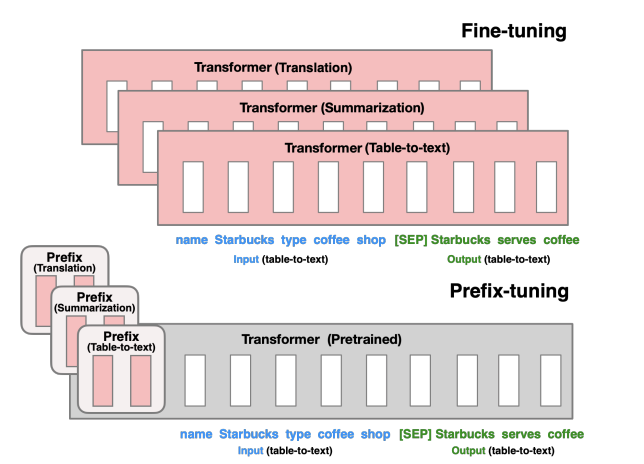
\includegraphics[width=0.8\textwidth]{chapter-2/prefix-tuning.png}
    \caption{Arsitektur \textit{Prefix-Tuning} \parencite{prefix_tuning}}
    \label{fig:prefix-tuning}
\end{figure}

Keuntungan utama dari pendekatan ini adalah efisiensi. Dengan mengoptimalkan hanya sebagian kecil dari parameter, \textit{Prefix-Tuning} dapat mencapai peningkatan kinerja dengan \textit{overhead} komputasi yang jauh lebih rendah dibandingkan dengan teknik \textit{fine-tuning} tradisional. Selain itu, dengan fokus pada \textit{prefix}, teknik ini memungkinkan adaptasi yang lebih spesifik terhadap tugas atau domain tertentu, memberikan fleksibilitas lebih dalam aplikasi praktis.

Teknik ini dapat digunakan untuk meningkatkan kinerja model generatif di berbagai tugas, termasuk penerjemahan mesin, peringkasan teks, dan lainnya. Hasil eksperimen menunjukkan bahwa \textit{Prefix-Tuning} mampu mencapai kinerja yang sebanding atau bahkan lebih baik dibandingkan dengan metode \textit{fine-tuning} tradisional, tetapi dengan biaya komputasi yang jauh lebih rendah.

